\documentclass[parskip]{scrartcl}
\usepackage{preamble}

% Title Page
% Definitionen für die Titelseite
% Change the content of the second bracket pair to what you need
\newcommand{\workauthor}{YOUR NAME}
\newcommand{\worktitle}{ESSAY TITLE}
\newcommand{\studentid}{123456}
\newcommand{\workyear}{YEAR}
\newcommand{\supervisor}{SUPERVISOR}
\newcommand{\shortabstract}{SHORT ABSTRACT}
\newcommand{\paper}{CITATION OF YOUR PAPER}

\begin{document}

\begin{titlepage}
    % HIER NICHTS ÄNDERN SONDER BEI DEN DEFINITIONEN OBEN DRÜBER    
    {\usekomafont{title}
    {\vspace*{1cm}\Huge \worktitle{}}}
    
    \vspace{\stretch{2}}
    
    {\Large \workauthor{}}
    
    Student ID: \studentid{}
    
    \vspace{\stretch{6}}
    
    Seminar Scientific Essay Writing and Presentations Skills Summer Term \workyear{}
    
    Supervisor: \textbf{\supervisor{}}
    
    \vspace{\stretch{4}}
    
    \shortabstract{}
    
    \vspace{\stretch{4}}
    
    Based on the Article:
    
    \paper{}
    
\end{titlepage}




\begin{abstract}

    The full abstract goes here
    

\end{abstract}



\tableofcontents

%    Abkürzungsverzeichnis
{\setlength{\parskip}{0.2cm}
\section*{Abbreviations}
    \begin{acronym}[LC-MS/MS23]
        % A B C D E F G H I J K L M N O P Q R S T U V W X Y Z        
        % Abkürzungen
        \acro{GABA}{\textgreek{g}-Aminobutyric acid}
        
        % Formelzeichen
        
        
        % als benutzt markierte Acronyme    
        
        
    \end{acronym}
}
\section{Introduction}\label{sec:introduction}
Your introduction goes here! Dummy citation: \cite{Alberts.2015}

\subsection{Dummy figure sub-section}\label{ssec:Dummyfiguresub-section}

\begin{figure}[h]%hbpt!H are options for figure placement
    \centering
    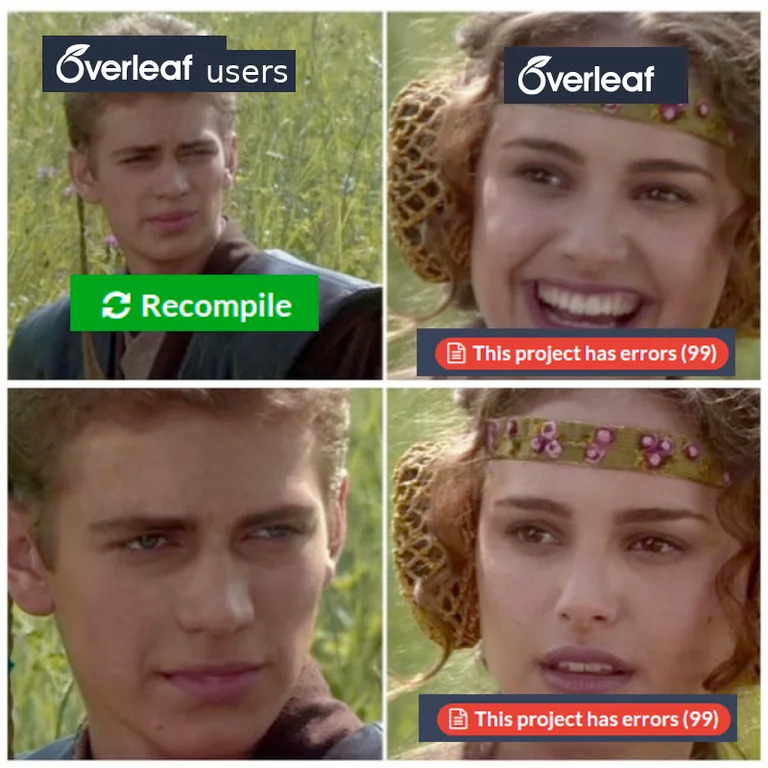
\includegraphics[width=.5\textwidth]{fig/overleaf.jpg}
    \caption{\textbf{A meaningful caption title.} This figure shows why compiling is always an option.}
    \label{fig:Ameaningfullcaption}
\end{figure}

\begin{table}[h]%hbpt!H are options for figure placement
    \centering
    \caption{\textbf{A dummy table.} You can use it as template for other tables. Remember caption goes on top because figure is bottom.}
    \label{tab:Thisisadummytable}
        \begin{tabular}{lcc} % l, r,c are options for alignments of a column, a | introduces vertical lines.
            \toprule
            \textbf{I}       &   \textbf{am}   &   \textbf{Head}    \\
            \midrule
            value   &   1    &   2       \\
            value   &   1    &   2       \\
            value   &   1    &   2       \\
            \bottomrule
        \end{tabular}
\end{table}


In the text we can do see: \Fref{fig:Ameaningfullcaption} or \sFref{fig:Ameaningfullcaption} and please look at \Tref{tab:Thisisadummytable} or \sTref{tab:Thisisadummytable}.

\section{Material and Methods}
	\paragraph{Method A}
		Your methods go here as paragraphs.

\section{Results}
	\subsection{Result for Method A}
		Results go here as subsections.
		
\section{Discussion}
	Your Discussion goes here!
	
\newpage
\printbibliography
\end{document}

